\xiaojie

一、视图是利用正投影的原理画出的。
正投影的概念是从日常生活中的“影子”加以科学的抽象而得出的。
正投影与光线下物体的“影子”是有区别的,它不是黑的阴影,而是通过规定的线型来表现的,
无论是看得见,或看不见的轮廓线,都要在图上反映出来。
如图 \ref{fig:czjh2-8-22},左图是一般的“影子”,右图是正投影。

在阳光下射线与投影面垂直是很少见的,但正投影概念里投射线与投影面是垂直的。


二、平面形的正投影是画简单几何体视图的基础,平面形的正投影规律是:
平行形不变,倾斜形改变,垂直成线段。

\begin{figure}[htbp]
    \centering
    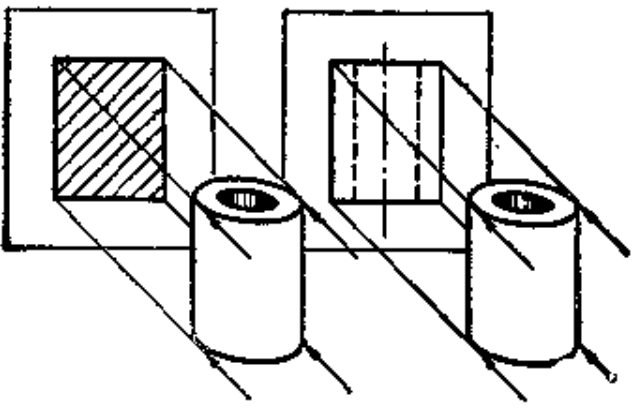
\includegraphics[width=11cm]{../pic/czjh2-ch8-22.png}
    \caption{}\label{fig:czjh2-8-22}
\end{figure}


三、一些形状复杂的物体可以看成是由简单体切割和组合而成的,掌握了简单体的画法规则后,
就容易掌握这些复杂形体的画法规则。

二视图是学习三视图的基础。对于三视图要注意:长对正,宽相等,高平齐。


四、画视图时,要注意正确运用线型,正确标注尺寸,同时要根据比例尺画图。

